%compile with pdflatex on papeeria

\documentclass[a4paper,12pt]{article}


\usepackage{fontawesome}

\usepackage{fancyhdr}
\usepackage{fancyheadings}
\usepackage[ngerman,german]{babel}
\usepackage{german}
\usepackage[utf8]{inputenc}
%\usepackage[latin1]{inputenc}
\usepackage[active]{srcltx}
%\usepackage{algorithm}
%\usepackage[noend]{algorithmic}
\usepackage{amsmath}
\usepackage{amssymb}
\usepackage{amsthm}
\usepackage{bbm}
\usepackage{enumerate}
\usepackage{graphicx}
\usepackage{ifthen}
\usepackage{listings}
\usepackage{enumitem}
%\usepackage{struktex}
\usepackage{hyperref}
\usepackage{tikz}
\usepackage{float}
\usepackage{subcaption}
\usepackage{array}
\captionsetup{compatibility=false}
\captionsetup[subfigure]{labelformat=empty}

\usepackage{pgfplots}
\pgfplotsset{compat=1.15}
\usepackage{mathrsfs}
\usetikzlibrary{arrows}

\definecolor{ccqqqq}{rgb}{0.8,0,0}
\definecolor{kolorwykresu}{rgb}{0.07,0.04,0.56}

\pagenumbering{gobble}

\usepackage{tabularray}
\usepackage{multirow}
\usepackage{booktabs,tabularx}

\DeclareMathSymbol{\shortminus}{\mathbin}{AMSa}{"39}

\renewcommand\tabularxcolumn[1]{m{#1}}% for vertical centering text in X column

\newcolumntype{L}[1]{>{\raggedright\let\newline\\\arraybackslash\hspace{0pt}}m{#1}}
\newcolumntype{C}[1]{>{\centering\let\newline\\\arraybackslash\hspace{0pt}}m{#1}}
\newcolumntype{R}[1]{>{\raggedleft\let\newline\\\arraybackslash\hspace{0pt}}m{#1}}

\newcolumntype{Y}{>{\centering\arraybackslash}X}

%%%%%%%%%%%%%%%%%%%%%%%%%%%%%%%%%%%%%%%%%%%%%%%%%%%%%%
%%%%%%%%%%%%%% EDIT THIS PART %%%%%%%%%%%%%%%%%%%%%%%%
%%%%%%%%%%%%%%%%%%%%%%%%%%%%%%%%%%%%%%%%%%%%%%%%%%%%%%
\newcommand{\Fach}{2. Schulaufgabe aus der Mathematik}
\newcommand{\Name}{}
\newcommand{\datum}{}
\newcommand{\Matrikelnummer}{}
\newcommand{\Semester}{7G}
\newcommand{\Uebungsblatt}{} %  <-- UPDATE ME
%%%%%%%%%%%%%%%%%%%%%%%%%%%%%%%%%%%%%%%%%%%%%%%%%%%%%%
%%%%%%%%%%%%%%%%%%%%%%%%%%%%%%%%%%%%%%%%%%%%%%%%%%%%%%

\setlength{\parindent}{0em}
\topmargin -1.0cm
\oddsidemargin 0cm
\evensidemargin 0cm
\setlength{\textheight}{9.2in}
\setlength{\textwidth}{6.0in}

%%%%%%%%%%%%%%%
%% Aufgaben-COMMAND
\newcommand{\Aufgabe}[1]{
  {
  \vspace*{0.5cm}
  \textsf{\textbf{Aufgabe #1}}
  \vspace*{0.2cm}
  
  }
}
%%%%%%%%%%%%%%
\hypersetup{
    pdftitle={\Fach{}: Übungsblatt \Uebungsblatt{}},
    pdfauthor={\Name},
    pdfborder={0 0 0}
}

\lstset{ %
language=java,
basicstyle=\footnotesize\tt,
showtabs=false,
tabsize=2,
captionpos=b,
breaklines=true,
extendedchars=true,
showstringspaces=false,
flexiblecolumns=true,
}

\newcommand*{\quadratbox}{\textbf{\fbox{\phantom{\huge{?}}}}}%

\title{Übungsblatt \Uebungsblatt{}}
\author{\Name{}}

\begin{document}

\fancyhead{}
\fancyhead[C]{
\includegraphics[height=2.5cm]{lukasLogo.png}
\vspace{2cm}
}

\thispagestyle{fancy}

\lhead{
%\vspace{1cm}
  \sf \LARGE \Fach{} %\small \Name{} - \Matrikelnummer{}
}
\rhead{\sf \Semester{}   \datum{}}

\vspace*{0.2cm}

\vspace{4cm}
Alle Lösungen müssen mit Nebenrechnungen und Begründungen nachvollziehbar sein!

%\rhead{\sf \Semester{} }
\vspace*{0.2cm}

%\begin{center}
%%\LARGE \sf \textbf{Übungsblatt \Uebungsblatt{}}
%\end{center}
%\vspace*{0.2cm}

%%%%%%%%%%%%%%%%%%%%%%%%%%%%%%%%%%%%%%%%%%%%%%%%%%%%%%
%% Insert your solutions here %%%%%%%%%%%%%%%%%%%%%%%%
%%%%%%%%%%%%%%%%%%%%%%%%%%%%%%%%%%%%%%%%%%%%%%%%%%%%%%

\vspace{1cm}
  Name: \underline{\hspace{7cm}}
  \hfill
  Datum: \underline{\hspace{4cm}}

\vspace{0.8cm}

\textbf{Hinweise:} Der Lösungsweg muss nachvollziehbar sein. Arbeitszeit \textbf{45 Minuten}.
%\vspace{0,5cm}Die Rechenwege müssen nachvollziehbar sein!
%
%\vspace{0,5cm} {TEIL A} - ohne Hilfsmittel - Bearbeitungszeit 30 Minuten
\vspace {0.8cm}
% 
%GEOMETRIE


\begin{center}
  \begin{tblr}{
      width=1\linewidth,
      colspec = {Q[c,6em]Q[c,4em]Q[c,4em]Q[c,4em]Q[c,4em]Q[c,4em]Q[c,6em]Q[c,6em]},
      rowspec = {Q[m]Q[m]Q[m]Q[m]Q[m]Q[m]Q[m]Q[m]},
      colsep = 0mm,
      %row{1} = {2em,azure2,fg=white,font=\large\bfseries\sffamily},
      row{1} = {2em,font=\large\bfseries\sffamily},
      hlines, vlines,
    }
    \textbf{Aufgabe} & \textbf{1} & \textbf{2} & \textbf{3} & 
    \textbf{4} & \textbf{5} & \textbf{Gesamt} & \textbf{Note}\\
    {Mögliche \\ Punkte} & {8} & {5} & {3} & 7 & 11 & {34} & \\
    {Erreichte \\ Punkte} &  &  &  &  & & &  \\
  \end{tblr}
\end{center}

\vspace{1cm}
%\centerline{\huge\bfseries\sffamily Viel Erfolg !!!}

%\newpage
%\vspace*{-2cm}
\Aufgabe{1: (4BE + 4BE)}
Vereinfache die Terme so weit wie möglich. Verwende dabei die binomischen
Formeln, wenn möglich.

\begin{enumerate}[label={\alph*)}]
  \item $(a-3)(a+3) -3(2a+5)^2=$
    \vspace{30mm}
    \newpage
\vspace*{-2cm}
  \item $x:\frac{5}{24}-(25x-15)^2:5+0,2x(x+3)-2,6=$
    \vspace{50mm}
\end{enumerate}

\Aufgabe{2: (5BE)}

Ersetze jeweils den/die Platzhalter, sodass äquivalente Terme enstehen.

\begin{enumerate}[label={\alph*)}]
  \item $\quadratbox x+4y=-2(3x-2y)$
  \item $\quadratbox a^2-\quadratbox ab = - \frac{a}{3}(2a+6b)$
  \item $\frac{15}{6}x-\frac{5}{3}y=\frac{5}{6}(\quadratbox x - \quadratbox y)$
\end{enumerate}


\Aufgabe{3: (3BE)}

\begin{minipage}[t]{0.55\textwidth}
Begründe, warum nebenstehende Konstruktion einer Mittelsenkrechten falsch ist und \underline{beschreibe} wie man sie richtig konstruiert.
\end{minipage}
\hspace*{2.05cm}
\begin{minipage}[t]{0.55\textwidth}
  \begin{figure}[H]
    \vspace{-1cm}
    \centering
    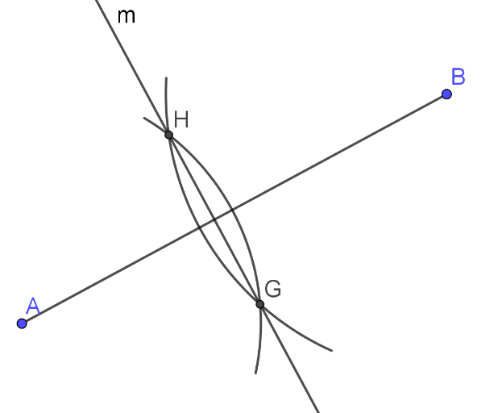
\includegraphics[width=0.7\linewidth]{7G_2SA_image1.png}
  \end{figure}
\end{minipage}


\newpage
\vspace*{-2cm}
\Aufgabe{4: (3BE + 2BE + 2BE)}
\begin{enumerate}[label={\alph*)}]
  \item Trage die Punkte $A(1|2)$, $B(6|0)$, $C(3|3)$, $D(-1|4)$, $E(4|-1)$ und $F(-3|1)$ in ein Koordinatensystem ein. (Koordinatensystem $-6\le x \le 6$, $-6\le y \le 6$)\\ 
    Konstruiere das Spiegelbild des Dreiecks $ABC$ an der Spiegelachse $DE$. 
  \item Konstruiere einen Lot auf die Gerade $DE$ durch Punkt $F$.
\vspace{190mm}
  \item Gib die Größe und Art der Winkel $\angle ABC$ und $\angle FAD$
\vspace{50mm}
\end{enumerate}

\newpage
\vspace*{-2cm}

\Aufgabe{5: (2BE + 3BE + 3BE + 3BE)}

\begin{minipage}[t]{0.55\textwidth}
  Herr Gärtner möchte seinen $a$ Meter langen und $b$ Meter breiten Garten mit Wegen versehen, wobei die Wege jeweils $0,6$ Meter breit sind. Er hat sich vier Möglichkeiten aufgezeichnet. \\
  (Skizze ist nicht maßstabsgetreu)
\end{minipage}
\hspace*{0.75cm}
\begin{minipage}[t]{0.40\textwidth}
  \begin{figure}[H]
    \vspace{-1cm}
    \centering
    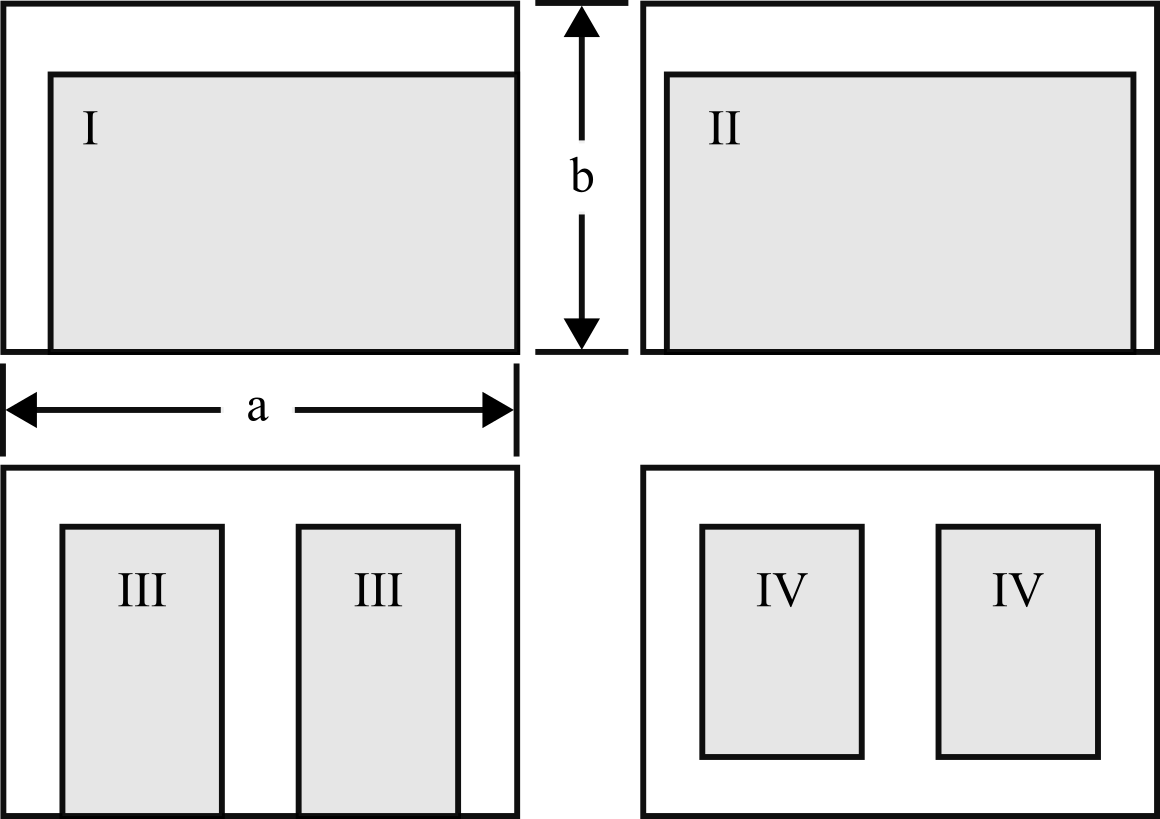
\includegraphics[width=1\linewidth]{7G_2SA_image2.png}
  \end{figure}
\end{minipage}
\begin{enumerate}[label={\alph*)}]
  \item Ordne der I. und II. Möglichkeit jeweils den richtigen Term für die Blumenbeetfläche (graue Bereiche) zu.


\begin{minipage}[t]{0.45\textwidth}
    \begin{enumerate}[label=\arabic*.]
    \item $(a-0,6)\cdot (b-1,8)$
    \item $(a-1,8)\cdot (b-0,6)$
    \item $(a-0,6)\cdot (b-0,6)$
  \end{enumerate}
\end{minipage}
\hspace*{0.15cm}
\begin{minipage}[t]{0.35\textwidth}
    \begin{enumerate}[label=\arabic*.]
    \setcounter{enumii}{3}
    \item $(a-1,2)\cdot (b-0,6)$
    \item $(a-1,2)\cdot (b-1,2)$
    \item $(a-1,8)\cdot (b-1,2)$
  \end{enumerate}
\end{minipage}
    \vspace{10mm}


  \item Berechne die Größe der III. Blumenbeetfläche, wenn $a=7,2m$ und $b=5,8m$ ist.
    \vspace{50mm}
  \item Herr Gärtner will einen kleinen Zaun um die beiden Blumenbeete bei der Option IV bauen. Er hat dafür $40m$ Zaun gekauft. Berechne ob das ausreichend ist, wenn Länge und Breite des gesamten Gartens so wie bei der Aufgabe b) sind.
    \vspace{50mm}
  \item Stelle einen Term für den Flächeninhalt aller Wege der IV. Möglichkeit in Abhängigkeit von $a$ und $b$ auf.
\end{enumerate}

%\begin{enumerate}[label={\alph*)}]

\vspace{1cm}

%\Aufgabe{5: }
%Ronja behauptet, dass die Terme $(3x - y)^2$ und $(y - 3x)^2$ äquivalent sind. Überprüfe diese Behauptung und begründe Deine Antwort.



%\vspace{3cm}
%\centerline{Viel Erfolg \faThumbsOUp }
\end{document}
